\documentclass[12pt]{article}
\usepackage[utf8]{inputenc}
\usepackage{float}
\usepackage{amsmath}
\usepackage{kbordermatrix}
\usepackage{amssymb}

\usepackage{tikz}
\usepackage{forest}
\usetikzlibrary{positioning}

\usepackage[hmargin=3cm,vmargin=6.0cm]{geometry}
%\topmargin=0cm
\topmargin=-2cm
\addtolength{\textheight}{6.5cm}
\addtolength{\textwidth}{2.0cm}
%\setlength{\leftmargin}{-5cm}
\setlength{\oddsidemargin}{0.0cm}
\setlength{\evensidemargin}{0.0cm}

%misc libraries goes here
\usepackage{fitch}

\begin{document}

\section*{Student Information } 
%Write your full name and id number between the colon and newline
%Put one empty space character after colon and before newline
Full Name :  Alperen OVAK\\
Id Number :  2580801\\

% Write your answers below the section tags
\section*{Answer 1}

\begin{figure}[H] 
    \[
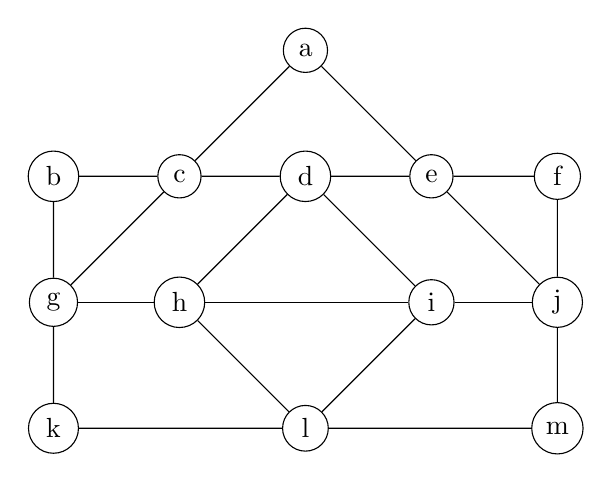
\begin{tikzpicture}[scale=0.8]
    \node[circle,draw] (a) at (0,4) {a};
    \node[circle,draw] (b) at (-4,2) {b};
    \node[circle,draw] (c) at (-2,2) {c};
    \node[circle,draw] (d) at (0,2) {d};
    \node[circle,draw] (e) at (2,2) {e};
    \node[circle,draw] (f) at (4,2) {f};
    \node[circle,draw] (g) at (-4,0) {g};
    \node[circle,draw] (h) at (-2,0) {h};
    \node[circle,draw] (i) at (2,0) {i};
    \node[circle,draw] (j) at (4,0) {j};
    \node[circle,draw] (k) at (-4,-2) {k};
    \node[circle,draw] (l) at (0,-2) {l};
    \node[circle,draw] (m) at (4,-2) {m};
    \draw (a) -- (e) -- (j);
    \draw (a) -- (c) -- (g);
    \draw (d) -- (h) -- (l) -- (i) -- (d);
    \draw (b) -- (g) -- (k);
    \draw (f) -- (j) -- (m);
    \draw (b) -- (c) -- (d) -- (e) -- (f);
    \draw (g) -- (h) -- (i) -- (j);
    \draw (k) -- (l) -- (m);
\end{tikzpicture}
\]
\caption{Graph G in \(Q_1\)}
\end{figure}

\subsection*{a)}

For a graph to have an Eulerian circuit, each vertex must have an even degree (number of edges incident to it), and the graph must be connected (Theorem 1, Section 10.5).

From the graph \( G \) provided:

\begin{itemize}
    \item Vertex \( a \) has degree 2.
    \item Vertex \( b \) has degree 2.
    \item Vertex \( c \) has degree 4.
    \item Vertex \( d \) has degree 4.
    \item Vertex \( e \) has degree 4.
    \item Vertex \( f \) has degree 2.
    \item Vertex \( g \) has degree 4.
    \item Vertex \( h \) has degree 4.
    \item Vertex \( i \) has degree 4.
    \item Vertex \( j \) has degree 4.
    \item Vertex \( k \) has degree 2.
    \item Vertex \( l \) has degree 4.
    \item Vertex \( m \) has degree 2.
\end{itemize}

All vertices have even degrees, which means graph \( G \) meets the first criterion.

The graph \( G \) is also connected as you can see in the graph, as we can trace a path from any vertex to any other vertex in the graph by following the edges.

Here is an Eulerian circuit: \\

\( k-g-b-c-a-e-f-j-m-e-i-j-e-d-i-h-d-c-g-h-l-k \) \\

Therefore, graph \( G \) does have an Eulerian circuit.


\subsection*{b)}

For an Eulerian path (that is not a circuit) to exist, the number of vertices which have odd degree must be 2 (Theorem 2, Section 10.5). Additionally, the graph must be connected.

Since there is no odd degreed vertices, we can say that there is no an Eulerian path.

\subsection*{c)}

To determine if graph \( G \) has a Hamiltonian circuit, we must find a closed loop that visits each vertex exactly once and returns to the starting vertex.

\textbf{Observations and Analysis:}

\begin{itemize}
    \item \textbf{Vertex Degrees:} The vertices \( a \), \( b \), \( f \), \( k \), and \( m \) have a degree of 2. In a Hamiltonian circuit, we must use all edges connected to vertices of degree 2, entering and exiting each of these vertices (Conditions for the Existence of Hamilton Circuits, Section 10.5).
    
    \item \textbf{Outer Circle Formation:} When we consider the edges connected to vertices of degree 2 and ensure that we enter and exit each of these vertices, we form an outer circle or loop. This outer loop includes edges connected to vertices \( a \), \( c \), \( b \), \( g \), \( k \), \( l \), \( m \), \( j \), \( f \) and \( e \).
    \begin{figure}[H] 
        \[
    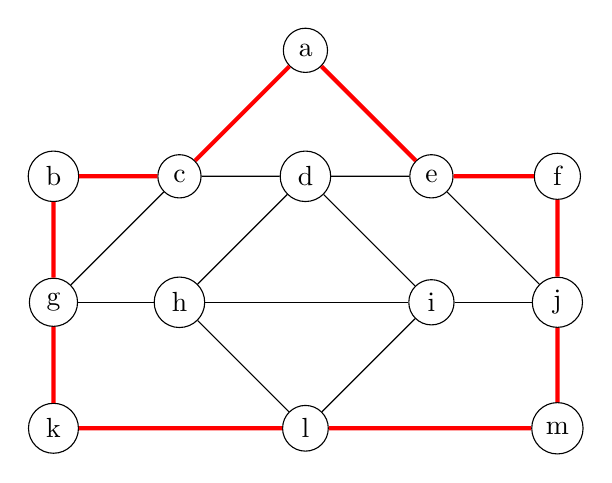
\begin{tikzpicture}[scale=0.8]
        \node[circle,draw] (a) at (0,4) {a};
        \node[circle,draw] (b) at (-4,2) {b};
        \node[circle,draw] (c) at (-2,2) {c};
        \node[circle,draw] (d) at (0,2) {d};
        \node[circle,draw] (e) at (2,2) {e};
        \node[circle,draw] (f) at (4,2) {f};
        \node[circle,draw] (g) at (-4,0) {g};
        \node[circle,draw] (h) at (-2,0) {h};
        \node[circle,draw] (i) at (2,0) {i};
        \node[circle,draw] (j) at (4,0) {j};
        \node[circle,draw] (k) at (-4,-2) {k};
        \node[circle,draw] (l) at (0,-2) {l};
        \node[circle,draw] (m) at (4,-2) {m};
        \draw (j) -- (e) edge[red, line width=1.5pt] (a);
        \draw (g) -- (c) edge[red, line width=1.5pt] (a);
        \draw (d) -- (h) -- (l) -- (i) -- (d);
        \draw (b) edge[red, line width=1.5pt] (g) ;
        \draw (g) edge[red, line width=1.5pt] (k);
        \draw (f) edge[red, line width=1.5pt] (j);
        \draw (j) edge[red, line width=1.5pt] (m);
        \draw (d) -- (c) edge[red, line width=1.5pt] (b);
        \draw (d) -- (e) edge[red, line width=1.5pt] (f);
        \draw (g) -- (h) -- (i) -- (j);
        \draw (k) edge[red, line width=1.5pt] (l);
        \draw (l) edge[red, line width=1.5pt] (m);
    \end{tikzpicture}
    \]
\caption{Outer loop of graph G after connecting  to vertices with degree 2}
\end{figure}
    \item \textbf{Inner Vertices:} The vertices which are not visited in the outer loop are \( d \), \( h \) and \( i \). To form a Hamiltonian circuit, we must also visit these inner vertices exactly once.But, we know that a Hamilton circuit cannot contain a smaller circuit within it (Conditions for the Existence of Hamilton Circuits, Section 10.5).
    
    \item \textbf{Revisiting Vertices:} The challenge arises when we try to connect the outer loop with the inner vertices without revisiting any vertex. Due to the connectivity of graph \( G \), it is not possible to visit all inner vertices without revisiting at least one vertex, breaking the condition for a Hamiltonian circuit.
\end{itemize}

Based on the structure of the graph \( G \) and the analysis above, we can conclude that there is no Hamiltonian circuit in graph \( G \). The inability to connect the outer loop with the inner vertices without revisiting a vertex confirms the absence of a Hamiltonian circuit in this graph.


\subsection*{d)}

We know that If G is a simple graph with n vertices with \(n \geq 3\) such that the
degree of every vertex in G is at least n/2, then G has a Hamilton circuit.(Dirac's Theorem, Section 10.5)\\

Moreover,If G is a simple graph with n vertices with \(n \geq 3\) such that
\( deg(u) + deg(v) \geq n \) for every pair of nonadjacent vertices u and v in G, then G has a
Hamilton circuit.(Ore's Theorem, Section 10.5)\\

Since both theorem do not satisfy, we can not directly say that there is a Hamilton circuit, therefore we can not say directly there is a Hamilton Path. But we can also find a Hamilton Path manually.

Therefore there is a Hamilton path in G: \(  b - c - a - e - f - j - m - l - i-d-h-g-k \)

\subsection*{e)}

To determine the chromatic number \( \chi(G) \) of the graph \( G \):

\begin{enumerate}
    \item \textbf{Subgraph Analysis:} Consider the subgraph of \( G \) with the maximum size that forms a complete graph, \( K_3 \) (a triangle). This subgraph consists of vertices \( a \), \( b \), and \( c \). Given that \( K_3 \) requires 3 different colors to ensure no adjacent vertices share the same color, we know that at least 3 colors are necessary.
    
    \item \textbf{Degree and Chromatic Number Relation:} There's a relationship between the maximum degree of a graph and its chromatic number. Specifically, for a graph with maximum degree \( k \), it is \( (k+1) \)-colorable. In \( G \), the maximum degree is 4. Hence, by this relationship, \( G \) is \( (4+1) \)-colorable, implying \( G \) is 5-colorable.
    
    \item \textbf{Narrowing Down the Options:} Given the insights from the subgraph and the degree-chromatic number relationship, we know that \( 3 \leq \chi(G) \leq 5 \). To find the exact chromatic number, we can attempt to color the graph with 3 colors.
    
    \item \textbf{Verification:} By trying to color the graph \( G \) using only 3 colors, we can verify if it's possible to ensure no adjacent vertices share the same color. If successful, then \( \chi(G) = 3 \). If not, then \( \chi(G) \) would be 4 or 5.
\end{enumerate}

\begin{figure}[H] 
    \[
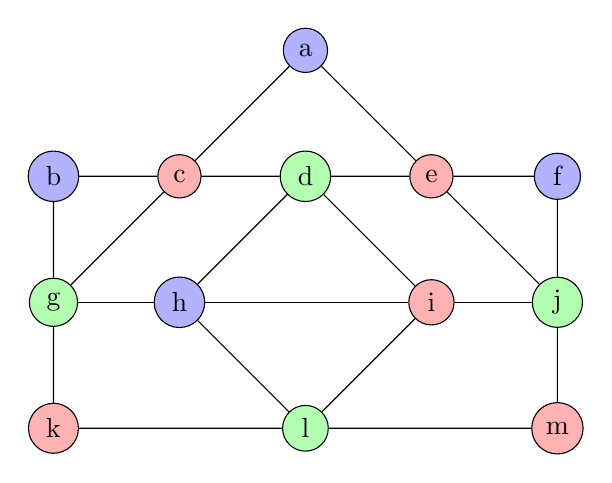
\begin{tikzpicture}[scale=0.8]
    \node[circle,draw,fill=blue!30] (a) at (0,4) {a};
    \node[circle,draw,fill=blue!30] (b) at (-4,2) {b};
    \node[circle,draw,fill=red!30] (c) at (-2,2) {c};
    \node[circle,draw,fill=green!30] (d) at (0,2) {d};
    \node[circle,draw,fill=red!30] (e) at (2,2) {e};
    \node[circle,draw,fill=blue!30] (f) at (4,2) {f};
    \node[circle,draw,fill=green!30] (g) at (-4,0) {g};
    \node[circle,draw,fill=blue!30] (h) at (-2,0) {h};
    \node[circle,draw,fill=red!30] (i) at (2,0) {i};
    \node[circle,draw,fill=green!30] (j) at (4,0) {j};
    \node[circle,draw,fill=red!30] (k) at (-4,-2) {k};
    \node[circle,draw,fill=green!30] (l) at (0,-2) {l};
    \node[circle,draw,fill=red!30] (m) at (4,-2) {m};
    \draw (a) -- (e) -- (j);
    \draw (a) -- (c) -- (g);
    \draw (d) -- (h) -- (l) -- (i) -- (d);
    \draw (b) -- (g) -- (k);
    \draw (f) -- (j) -- (m);
    \draw (b) -- (c) -- (d) -- (e) -- (f);
    \draw (g) -- (h) -- (i) -- (j);
    \draw (k) -- (l) -- (m);
\end{tikzpicture}
\]
\caption{Coloring of G with 3 different color}
\end{figure}

\textbf{Conclusion:}

After attempting to color the graph \( G \) with 3 colors, we find that it is indeed possible to do so without any adjacent vertices sharing the same color. Thus, the chromatic number \( \chi(G) \) of the graph \( G \) is 3.


\subsection*{f)}

\textbf{Chromatic Number and Bipartite Graphs:} 


A graph is bipartite if it's possible to color its vertices with just two distinct colors such that no neighboring vertices share the same color.(Theorem 4, Section 10.2)

It's correct that the chromatic number of a bipartite graph is 2. Since \( \chi(G) = 3 \) for \( G \), it confirms that \( G \) cannot be bipartite.\\

\textbf{Making \( G \) Bipartite:} To make \( G \) bipartite, we would aim to decrease its chromatic number to 2. This can be achieved by removing or "breaking" cycles of odd length in \( G \), as any such cycle in a graph prevents it from being bipartite.

<<<<<<< HEAD
\textbf{Removing \( K_3 \) Subgraphs:} We need to identify the \( K_3 \) subgraphs in \( G \). To make \( G \) bipartite by removing edges, we would focus on the \( K_3 \) subgraphs.
=======
\textbf{Removing \( K_3 \) Subgraphs:} Let's identify the \( K_3 \) subgraphs in \( G \). To make \( G \) bipartite by removing edges, we would focus on the \( K_3 \) subgraphs.\\

b-c-g, e-f-j, d-h-i and h-i-l are the \( K_3 \) subgraphs in \( G \).
>>>>>>> 8ea17215795011d6e1f2fe136cec27cf300e5d75

\begin{itemize}
    \item For \( K_3 \) subgraphs where all vertices are pairwise connected, removing any single edge would suffice.
    
    \item For \( K_3 \) subgraphs where two \( K_3 \) subgraphs share a common edge, removing just one edge would break both \( K_3 \) subgraphs into separate components.
\end{itemize}

Note that we need to create odd cycle.
The steps are so simple:
Select a random node to be the first object in set A. Choose one node to be the first in set B if there are any connected to it. If not, select any other node to be the set B's initial member.

Right now, A and B are our two sets of nodes. Select a node that is not in either set repeatedly. Determine how many edges connect that node to the nodes in A and B. Remove the edges connecting it to nodes in set B and place it in set B if there are further edges connecting it to set A. If not, insert it into set A and remove the edges connecting it to the nodes there.

Thus, \( b-c \), \( e-f \),\( h-i \) are the edges that should be deleted to get bipartite graph.

\begin{figure}[H] 
    \[
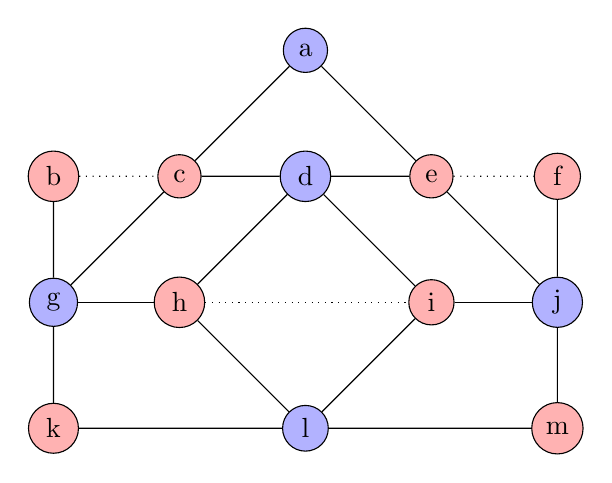
\begin{tikzpicture}[scale=0.8]
    \node[circle,draw,fill=blue!30] (a) at (0,4) {a};
    \node[circle,draw,fill=red!30] (b) at (-4,2) {b};
    \node[circle,draw,fill=red!30] (c) at (-2,2) {c};
    \node[circle,draw,fill=blue!30] (d) at (0,2) {d};
    \node[circle,draw,fill=red!30](e) at (2,2) {e};
    \node[circle,draw,fill=red!30] (f) at (4,2) {f};
    \node[circle,draw,fill=blue!30] (g) at (-4,0) {g};
    \node[circle,draw,fill=red!30] (h) at (-2,0) {h};
    \node[circle,draw,fill=red!30] (i) at (2,0) {i};
    \node[circle,draw,fill=blue!30] (j) at (4,0) {j};
    \node[circle,draw,fill=red!30] (k) at (-4,-2) {k};
    \node[circle,draw,fill=blue!30] (l) at (0,-2) {l};
    \node[circle,draw,fill=red!30] (m) at (4,-2) {m};
    \draw (a) -- (e) -- (j);
    \draw (a) -- (c) -- (g);
    \draw (d) -- (h) -- (l) -- (i) -- (d);
    \draw (b) -- (g) -- (k);
    \draw (f) -- (j) -- (m);
    \draw[dotted] (b) -- (c); 
    \draw (c)-- (d) -- (e);
    \draw[dotted] (e) -- (f);
    \draw (g) -- (h) ;
    \draw[dotted] (h) -- (i);cxxx
    \draw (i) -- (j);
    \draw (k) -- (l) -- (m);
\end{tikzpicture}
\]
\caption{Bipartite version of graph G after deleting the edges}
\end{figure}


\subsection*{g)}

We know that the chromatic number of a complete graph with n vertices is n (Example 2, Section 10.8).\\
Given the graph \( G \) with chromatic number \( \chi(G) = 3 \), it indicates that no set of four vertices in \( G \) can form a complete subgraph \( K_4 \), since a \( K_4 \) would require 4 distinct colors.

Upon examining the graph:

\begin{enumerate}
    \item Vertices \( d \), \( h \), and \( i \) form a complete subgraph \( K_3 \).
\end{enumerate}

To introduce a complete subgraph \( K_4 \) into \( G \), we need to add a vertex connected to \( d \), \( h \), \( i \), and \( l \).

The edge between vertices \( d \) and \( l \) can be added to \( G \) to ensure that the vertices \( d \), \( h \), \( i \), and \( l \) together form a complete subgraph \( K_4 \).

Thus, to incorporate a complete subgraph \( K_4 \) into \( G \), the edge connecting \( d \) and \( l \) should be added.

\begin{figure}[H] 
    \[
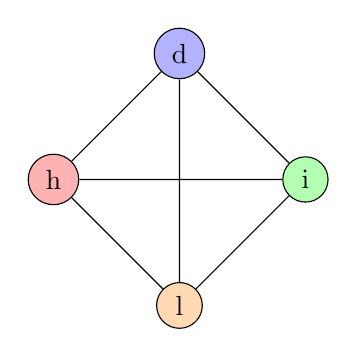
\begin{tikzpicture}[scale=0.8]

    \node[circle,draw,fill=blue!30] (d) at (0,2) {d};
    \node[circle,draw,fill=red!30] (h) at (-2,0) {h};
    \node[circle,draw,fill=green!30] (i) at (2,0) {i};
    \node[circle,draw,fill=orange!30] (l) at (0,-2) {l};

    \draw (d) -- (h) -- (l) -- (i) -- (d) -- (l) -- (i) -- (h);

\end{tikzpicture}
\]
\caption{subgraph \(K_4\) in G after adding the edge \{d,l\}}
\end{figure}

\section*{Answer 2}

Let's first verify some properties: the count of vertices, edges, and the number of vertices with each degree should match for both graphs. In graph \( G \), there are 8 vertices and 16 edges, with each vertex having a degree of 4. Similarly, in graph \( H \), there are also 8 vertices and 16 edges, and each vertex has a degree of 4. So, there is a possibility of isomorphism.

We need to introduce a function, \( i \) which is both one-to-one and onto, and then determine if it represents an isomorphism. By analyzing the cycles of lengths 3 and 4 in the graphs, we can define the following function, \( i \), by mapping the graphs: 
\begin{align*}
    i(a) = a',
    i(b) = c',
    i(c) = e', 
    i(d) = g', 
    i(e) = b', 
    i(f) = h', 
    i(g) = d', 
    i(h) = f'.
\end{align*}

We now have a one-to-one correspondence between the vertex set of \( G \) and the vertex set of \( H \).

Let's take a look at the adjacency matrix of \( G \):
\begin{figure}[H] 
\[
  \text{A}_{G} = \kbordermatrix{
    & a & b & c & d & e & f & g & h \\
    a & 0 & 1 & 0 & 1 & 1 & 1 & 0 & 0 \\ 
    b & 1 & 0 & 1 & 0 & 1 & 0 & 1 & 0 \\ 
    c & 0 & 1 & 0 & 1 & 0 & 0 & 1 & 1 \\ 
    d & 1 & 0 & 1 & 0 & 0 & 1 & 0 & 1 \\ 
    e & 1 & 1 & 0 & 0 & 0 & 1 & 0 & 1 \\ 
    f & 1 & 0 & 0 & 1 & 1 & 0 & 1 & 0 \\
    g & 0 & 1 & 1 & 0 & 0 & 1 & 0 & 1 \\
    h & 0 & 0 & 1 & 1 & 1 & 0 & 1 & 0 \\
  }
\]

\caption{Adjacency matrix of \( G \)}
\end{figure}


and the adjacency matrix of \( H \) with the rows and columns labeled by the images of the corresponding vertices in \( G \):
\begin{figure}[H] 
\[
  \text{A}_{H} = \kbordermatrix{
    & a' & c' & e' & g' & b' & h' & d' & f' \\
    a' & 0 & 1 & 0 & 1 & 1 & 1 & 0 & 0 \\ 
    c' & 1 & 0 & 1 & 0 & 1 & 0 & 1 & 0 \\ 
    e' & 0 & 1 & 0 & 1 & 0 & 0 & 1 & 1 \\ 
    g' & 1 & 0 & 1 & 0 & 0 & 1 & 0 & 1 \\ 
    b' & 1 & 1 & 0 & 0 & 0 & 1 & 0 & 1 \\ 
    h' & 1 & 0 & 0 & 1 & 1 & 0 & 1 & 0 \\
    d' & 0 & 1 & 1 & 0 & 0 & 1 & 0 & 1 \\
    f' & 0 & 0 & 1 & 1 & 1 & 0 & 1 & 0 \\
  }
\]
\caption{Adjacency matrix of \( H \)}
\end{figure}
Because \( A_G = A_H \), it follows that \( i \) preserves edges. We conclude that \( i \) is an isomorphism, so \( G \) and \( H \) are isomorphic.


\section*{Answer 3}

\subsection*{a)}

The chromatic number \( \chi(C_n) \) of the cycle graph \( C_n \) is 2 if \( n \) is even, and 3 if \( n \) is odd.



\textbf{ When \( n \) is even:}
For \( n \) even, we can see that the vertices of \( C_n \) can be alternately colored using two colors. To illustrate, consider \( C_6 \):

\begin{itemize}
    \item Start with vertex \( v_0 \) and color it red.
    \item Proceeding clockwise, the next vertex \( v_1 \) is colored blue.
    \item Continue this pattern, alternating between red and blue, until \( v_5 \), which is adjacent to \( v_0 \), is colored blue.
\end{itemize}
\begin{figure}[H] 
    \[
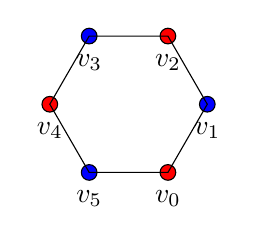
\begin{tikzpicture}
    % Vertices for C_6
    \foreach \x in {0,...,5} {
        \coordinate (v\x) at ({360/6 * (\x - 1)}:1);
        \ifodd\x
        \node[draw, circle, fill=blue, inner sep=2pt, label=below:{$v_\x$}] at (v\x) {};
        \else
          \node[draw, circle, fill=red, inner sep=2pt, label=below:{$v_\x$}] at (v\x) {};
        \fi
    }
    % Edges for C_6
    \draw (v0) -- (v1) -- (v2) -- (v3) -- (v4) -- (v5) -- cycle;
\end{tikzpicture}
\]
\caption{Coloring of \(Q_6\)}
\end{figure}

<<<<<<< HEAD

=======
>>>>>>> 8ea17215795011d6e1f2fe136cec27cf300e5d75
Thus, \( C_6 \) is bipartite and can be colored using two colors, indicating that the chromatic number is 2 and bipartite when \( n \) is even.

\textbf{When \( n \) is odd:}
For \( n \) odd, alternating colors while traversing \( C_n \) clockwise will eventually lead to a vertex (e.g., \( v_5 \) in \( C_5 \)) that is adjacent to both the starting vertex \( v_0 \) and the vertex before the starting vertex. This situation requires a third color to ensure no adjacent vertices share the same color.

For instance, in \( C_5 \):

\begin{itemize}
    \item Start with \( v_0 \) colored red.
    \item Proceeding clockwise, \( v_1 \) is blue, \( v_2 \) is red, \( v_3 \) is blue, but when reaching \( v_4 \), which is adjacent to both \( v_3 \) and \( v_0 \), a third color (say green) is needed.
\end{itemize}

\begin{figure}[H] 
    \[
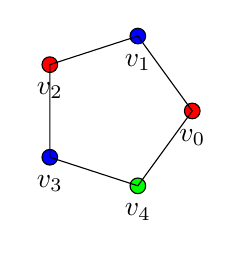
\begin{tikzpicture}
    % Vertices for C_5
    \foreach \x/\color in {0/red, 1/blue, 2/red, 3/blue, 4/green} {
      \coordinate (u\x) at ({360/5 * \x}:1);
      \node[draw, circle, fill=\color, inner sep=2pt, label=below:{$v_\x$}] at (u\x) {};
    }
    % Edges for C_5
    \draw (u0) -- (u1) -- (u2) -- (u3) -- (u4) -- cycle;
  \end{tikzpicture}
\]
\caption{Coloring of \(Q_5\)}
\end{figure}

Thus, \( C_5 \) requires three colors, indicating that the chromatic number is 3 and it is not bipartite when \( n \) is odd.


\subsection*{b)}

The chromatic number of the hypercube \( Q_n \) is 2. This can be understood by observing the binary nature of the vertex labels. We can partition the vertices into two sets based on the parity of the number of 1s in their binary labels:

\begin{itemize}
    \item One set contains vertices labeled with sequences having an even number of 1s.
    \item The other set contains vertices labeled with sequences having an odd number of 1s.
\end{itemize}

Within each set, vertices are not connected by edges because the Hamming distance between them would always be even. On the other hand, there will never be an edge between two sequences with the same parity (i.e., either both sequences have an even number of 1s or both have an odd number of 1s) because edges in \( Q_n \) exist only between sequences with binary labels that differ in one position (leading to a change in parity).

As we can understand that \( Q_n \) is a bipartite.

Thus, the vertices of \( Q_n \) can be colored with two colors in such a way that no two adjacent vertices have the same color, indicating that the chromatic number of \( Q_n \) is 2.


\section*{Answer 4}

\subsection*{a)}

In Kruskal's algorithm, we begin by selecting the edge in the graph with the smallest weight. We then proceed to add edges with the next smallest weights, ensuring that they don't create a loop with the previously chosen edges. The process concludes once we have chosen \( n - 1 \) edges.(Algorithm 2, Section 11.5)

The order in which the edges are added to the tree is \{a,b\}, \{c,e\},\{e,f\},\{a,d\},and \{b,c\}.

\begin{figure}[H] 

\begin{table}[H]
	\small
	\centering
	\begin{tabular}{|c|c|c|}	
	\hline
	$Choice$ & $Edge$ & $Weight$\\
	\hline 
	1 & $\{a,b\}$ & 1\\			
	2 & $\{c,e\}$ & 2\\	
	3 & $\{e,f\}$ & 2\\	
	4 & $\{a,d\}$ & 3\\	
	5 & $\{b,c\}$ & 4 \\	
	\hline 
	\end{tabular}
\end{table}

\caption{Table of Kruskal steps}
\end{figure}

\subsection*{b)}

\begin{figure}[H] 
    \[
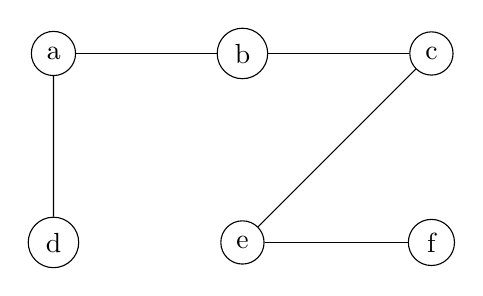
\begin{tikzpicture}[scale=0.8]
    \node[circle,draw,] (a) at (-3,0) {a};
    \node[circle,draw,] (b) at (0,0) {b};
    \node[circle,draw,] (c) at (3,0) {c};
    \node[circle,draw,] (d) at (-3,-3) {d};
    \node[circle,draw,](e) at (0,-3) {e};
    \node[circle,draw,] (f) at (3,-3) {f};
    
    \draw (a) -- (b);
    \draw (c) -- (e);
    \draw (e) -- (f);
    \draw (a) -- (d);
    \draw (b) -- (c);
    
\end{tikzpicture}
\]
\caption{Minimum spanning tree for the graph G}
\end{figure}

\subsection*{c)}

No, the choice isn't unique. For instance, selecting edge \{c,f\} would yield a similar cost as the one we initially picked in step-3. Hence, it leads to an alternative minimum spanning tree. The variations in minimum spanning trees arise due to the diverse selections made while applying the algorithm.

\begin{figure}[H] 
    \[
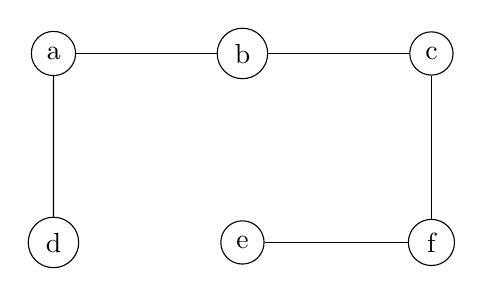
\begin{tikzpicture}[scale=0.8]
    \node[circle,draw,] (a) at (-3,0) {a};
    \node[circle,draw,] (b) at (0,0) {b};
    \node[circle,draw,] (c) at (3,0) {c};
    \node[circle,draw,] (d) at (-3,-3) {d};
    \node[circle,draw,](e) at (0,-3) {e};
    \node[circle,draw,] (f) at (3,-3) {f};
    
    \draw (a) -- (b);
    \draw (c) -- (f);
    \draw (e) -- (f);
    \draw (a) -- (d);
    \draw (b) -- (c);
    
\end{tikzpicture}
\]
\caption{Alternative spanning tree}
\end{figure}

\section*{Answer 5}

\subsection*{a)}

\textbf{Base Case (d = 1):}

Consider a full binary tree \( B_1 \) with depth 1. This tree consists of a single node (the root). The number of nodes \( N_1 \) is 1, and the number of leaves \( L_1 \) is also 1.

From the provided information:
\begin{align*}
N_1 &= 1 \\
L_1 &= \frac{N_1 + 1}{2} = \frac{2}{2} = 1
\end{align*}

The number of leaves satisfy the given formulas for the base case.

\textbf{Inductive Step (d \(\rightarrow\) d+1):}

Assume the statements hold for some full binary graph with \(n\) nodes and arbitrary depth \( d \). That is:
\begin{align*}
N_d &= n \\
L_d &= \frac{N_d + 1}{2}
\end{align*}

Now, consider a full binary tree \( B_{d+1} \) of depth \( d+1 \) with \( B_d \) as its last layer. Each leaf of \( B_d \) at depth \(d\) will have two leaves in \( B_{d+1} \) and they become a internal node.

1. \textbf{Nodes:} To obtain a full binary graph with depth \(d+1\) (\( B_{d+1} \)), for each leaf in \( B_d \) at depth \(d\), we can add 2 nodes in \( B_{d+1} \). Let's choose \(m\) many leaf where m is a positive integer, and add 2 leaf to each one. So, the new number of nodes \( N_{d+1} \) is:
\begin{align*}
N_{d+1} &= N_d + 2m \\
\end{align*}

2. \textbf{Leaves:} Each leaf in \( B_d \) at depth \(d\) transforms into two leaves in \( B_{d+1} \), and they become a internal node. Thus, the number of leaves \( L_{d+1} \) becomes:
\begin{align*}
L_{d+1} &= L_d + 2m - m\\
&= L_d + m \\
&= \frac{N_d + 1}{2} + m \\
&= \frac{N_d + 2m + 1}{2} \\
&= \frac{N_{d+1} + 1}{2} \\
\end{align*}
This matches the formula for \( L_{d+1} \).

Thus, both the number of nodes and leaves in the tree of depth \( d+1 \) satisfy the given formulas based on the induction hypothesis. This completes the inductive step.

By the principle of mathematical induction, the statements are true for all positive integers \( d \).


\subsection*{b)}

To show that the chromatic number of a tree is 2 using mathematical induction, we'll proceed with the following steps:

\textbf{Base Case:}
A tree with one vertex is trivially 2-colorable. Thus, the base case is true.\\

\textbf{Inductive Hypothesis:}
Assume that any tree with $n$ vertices is 2-colorable.\\

We want to prove that any tree with $n+1$ vertices is also 2-colorable.

Consider a tree $T$ with $n+1$ vertices. Remove any leaf vertex $v$ from $T$ to obtain a tree $T'$ with $n$ vertices.

Since $T'$ is a tree with $n$ vertices, by our inductive hypothesis, we can 2-color $T'$ such that no adjacent vertices have the same color.

Now, when we add the leaf vertex $v$ back to $T'$ to form $T$, we can always color $v$ with the color different from its adjacent vertex in $T'$ because $v$ is connected to only one other vertex in $T'$.

Thus, we can always 2-color the tree $T$ with $n+1$ vertices such that no adjacent vertices have the same color.

By the principle of mathematical induction, we can conclude that any tree can be 2-colored. Therefore, the chromatic number of a tree is 2.

\subsection*{c)}

The tree is called a full m-ary tree if every internal vertex has exactly m children.(Definition 3 - 11.1)

To get upper bound for height, we need to just add m children to one of the nodes in each level.

Therefore, we have m nodes in every level, except level-1. This means that the number of levels which have m many nodes equals to height of the tree.\\

So, we have total \( 1+mh = n \) nodes.

As a result, \( h \le \frac{n-1}{m}\)

It means that the upper bound of height is \( h=\frac{n-1}{m}\).

\begin{figure}[H] 
    \[
\begin{forest}
    for tree={circle, draw, minimum size=1em, s sep=10pt}
    [0
        [ 1  
            [2
                [3
                    [ \dots, edge label={node[midway,right,font=\tiny]{...}} ]
                ]
                [...]
                [...]
                [m]
            ]
            [...]
            [...]
            [m]
        ]
        [...]
        [...]
        [m]
    ]
    \end{forest}
\]
\caption{Full m-ary binary tree with m nodes in each level}
\end{figure}

\end{document}
